%update: Jan 13 fixed grammar according to prof notes
%update: Jan 09-11 prof check
%update: Dec 20 finish writing
%update: Nov 09 Prof checked some of the texts

%\begin{savequote}[75mm] 
%There's plenty of room at the bottom.
%\qauthor{Richard Feynman} 
%\end{savequote}

\setcounter{page}{1}
\pagenumbering{arabic}

\chapter{Introduction}

\newthought{The advancement of materials science and technology} has led to the discovery and utilization of nanoscale materials. Many of these new materials possess extraordinary chemical, electrical, optical or mechanical properties. However, as human beings, who are millions or billions times larger than nanomaterials, we are not perfectly scaled to reach them directly. As Feynman said, {\it there is plenty of room at the bottom}, but it also means that plenty of efforts are expected toward researching. 

\begin{figure} 
\centering
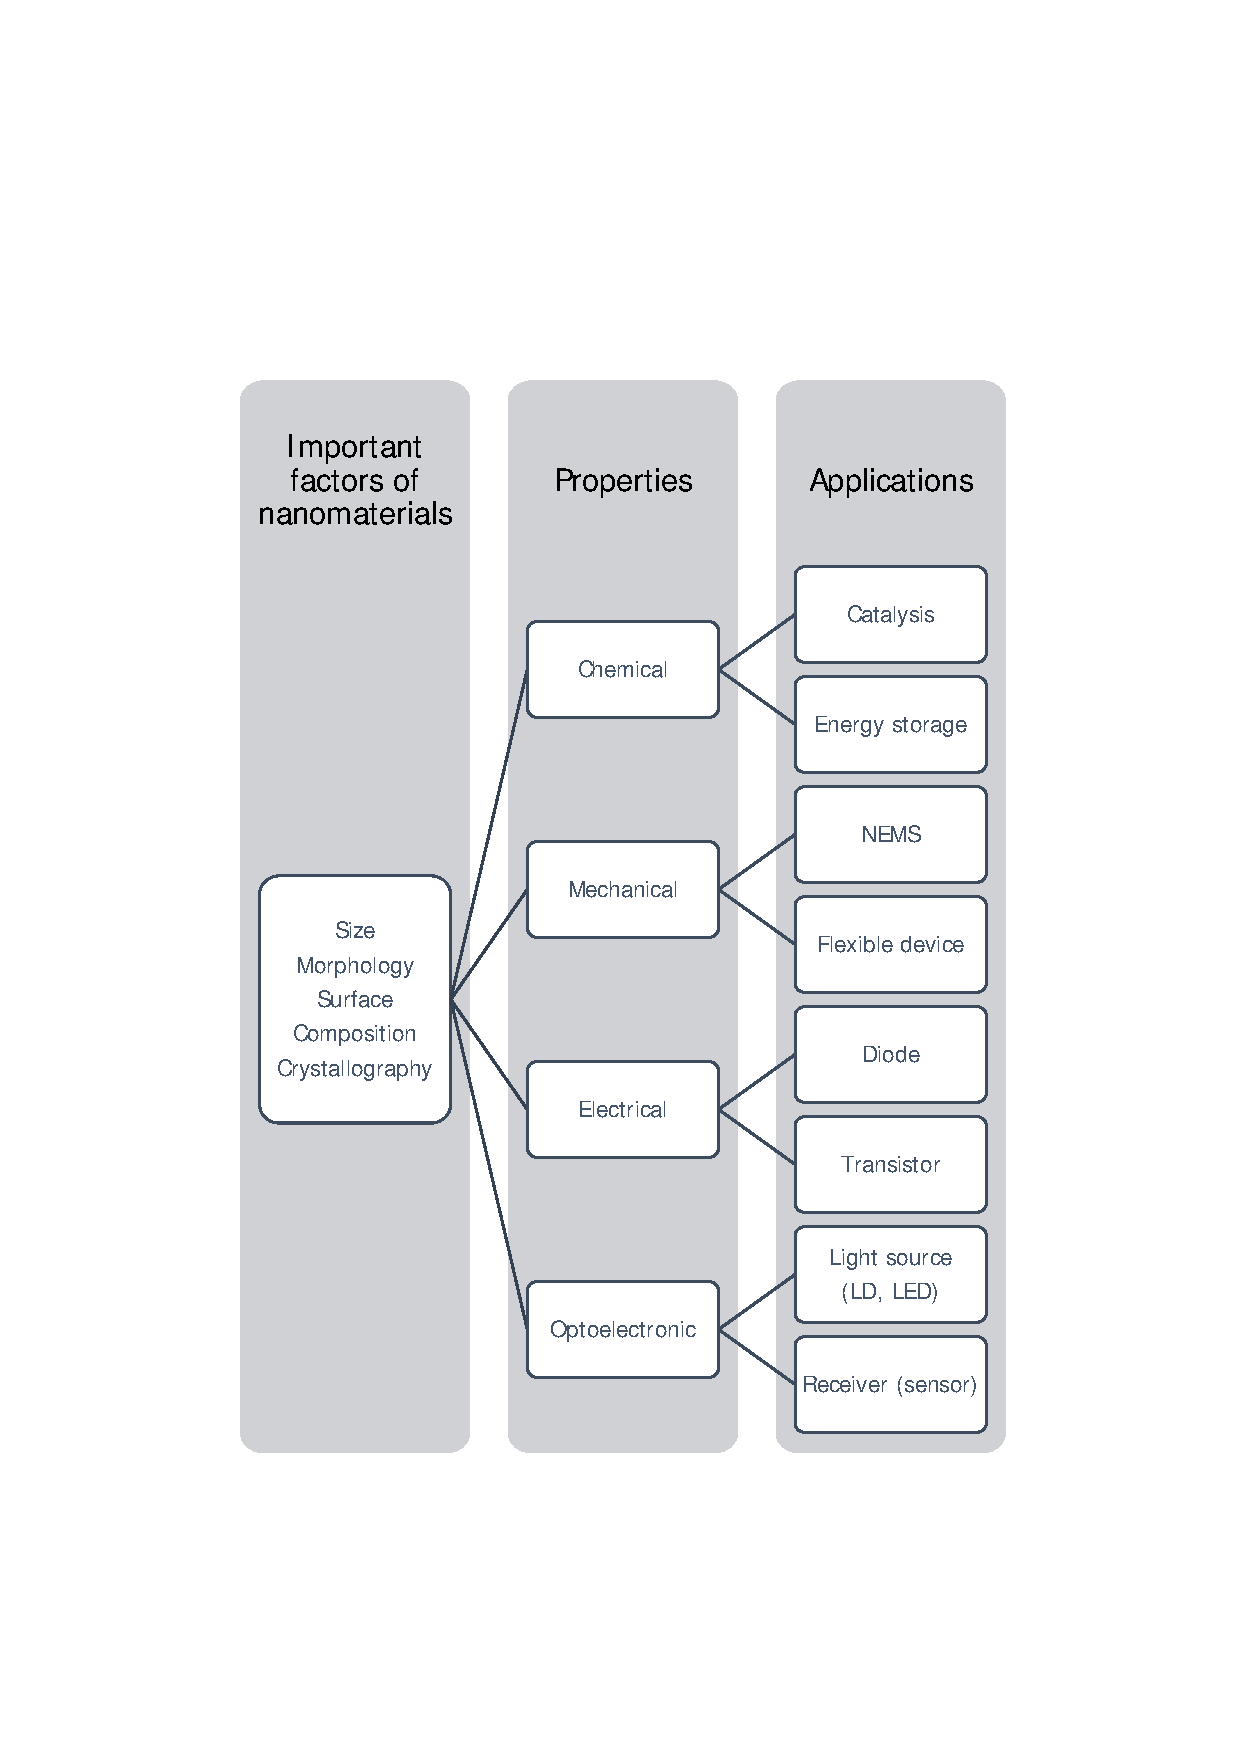
\includegraphics[width=400pt]{figures/figure1_factors}
\caption[Factors and applications]{Special factors of nanomaterials contributing to various applications. 
\label{fig:1_factor}}
\end{figure}

\section{Probing of nanomaterials}
Generally, nanomaterials are materials in which a single unit is sized from one nanometer to a few hundred nanometers. The scale difference between these materials and human body is more than a million. Besides scale difference, nanostructures usually possess special properties, as compared with bulk materials, due to chemical composition difference, surface to volume ratio and quantum confinements. The confined structures of the same chemical type and composition might present very different properties. An easy way to understand a value of the nanomaterial is to consider carbon materials. We know that diamond and graphite are allotropes of carbon which possess different bonding and thereby amazingly distinct physical and chemical characteristics. This is also true for a fullerene, a carbon nanotube and graphene. Even the number of walls in a carbon nanotube would significantly affect its properties. \cite{rodunerwhynano2006} Therefore, what makes nanostuctures distinctive is not only their size, but also their unique compositions, surfaces and quantum confinement effects. 

\renewcommand{\thefootnote}{\fnsymbol{footnote}}

As shown in Figure \ref{fig:1_factor}, many effects contribute to the particular functionality of a nanomaterial, such as superior mechanical strength and rigidity, ultrahigh electrical mobility, abundant chemical active sites, \textit{ect.} Mechanical superiority is important for applications, \textit{e.g.} for flexible electronics and devices in Nano Electro-Mechanical Systems (NEMS). Electrical superiority of nanomaterials with various electronic band structures could be applied in electrical diodes, transistors, laser diodes (LDs), light-emitting diodes (LEDs), and in transparent or flexible electronics and optoelectronics. Chemical superiority of nanomaterials make them desirable for highly efficient catalysis and portable energy storage devices with high energy density. 

\begin{figure} 
\centering
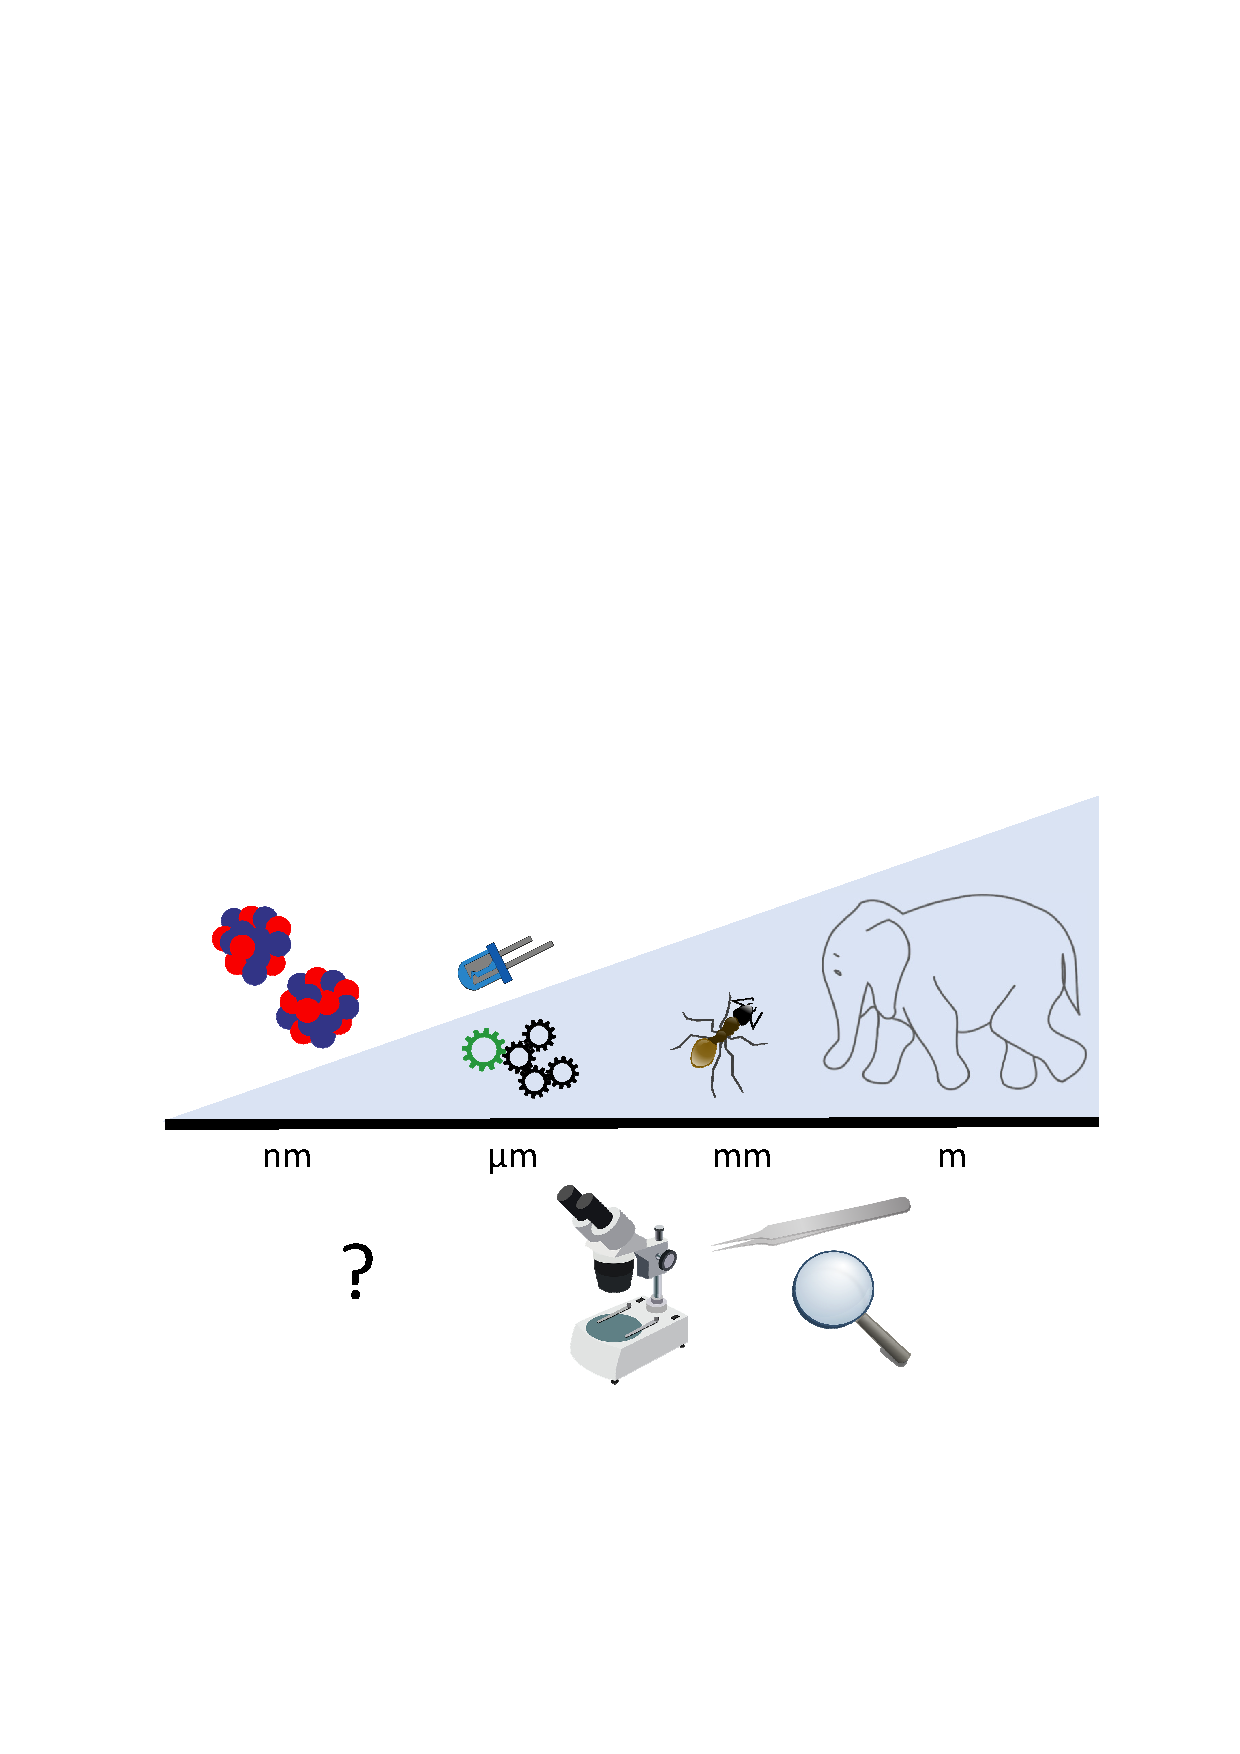
\includegraphics[width=\textwidth]{figures/figure1_scale_problem.pdf}
\caption[Scale problem]{How human beings gain access to lower scales, to see and to manipulate.\footnotemark[1]
\label{fig:1_scale}}
\end{figure}

However, it is not straightforward to access the properties of these nanomaterials and prepare them for real applications. Unfortunately, this is due to the above-mentioned issue - a small scale. We understand that the observation, reach and built of an object which is $10^6$ to $10^9$ (in one dimension) smaller then any real world macro-object, for example the {\em Great Wall of China} ($21,196 km$), is challenging. Similarly, as compared with human beings' hands, of a size is about 20 cm, nanoscaled objects are usually million times smaller. Hence, even though the nanoscale building blocks are superior in many respects in theory, we are not able to utilize them easily. As shown in Figure \ref{fig:1_scale} \footnote{Without specification, all clip art materials (elephant, ant, microscope, tweezers, etc.) in figures of the Dissertation are adapted from Internet which are {\em free to use without permission}.}, we are able to reach smaller scales using tweezers and optical microscopes, but it is very challenging to reach nanoscale objects. \\

The way human beings make use of fire, tools, light and electrons is perhaps what sets our modern live standards above of other species. By understanding and utilizing photons, electrons and atomic forces, microscopy allows us to view sub-millimeter objects that cannot be observed with a naked eye. Thanks to the advancement of tools - microscopy and piezoelectric materials - we can now access to nanomaterials by high precision probing technique under direct high-resolution observations. By applying electrical field to a piece of piezoelectric material, the latter precisely changes its shape in function of the applied electric field. Therefore, we may control the mechanical movements by electrical biases and confirm the location of an object and the probe using microscopy. 

\begin{figure}  
\centering
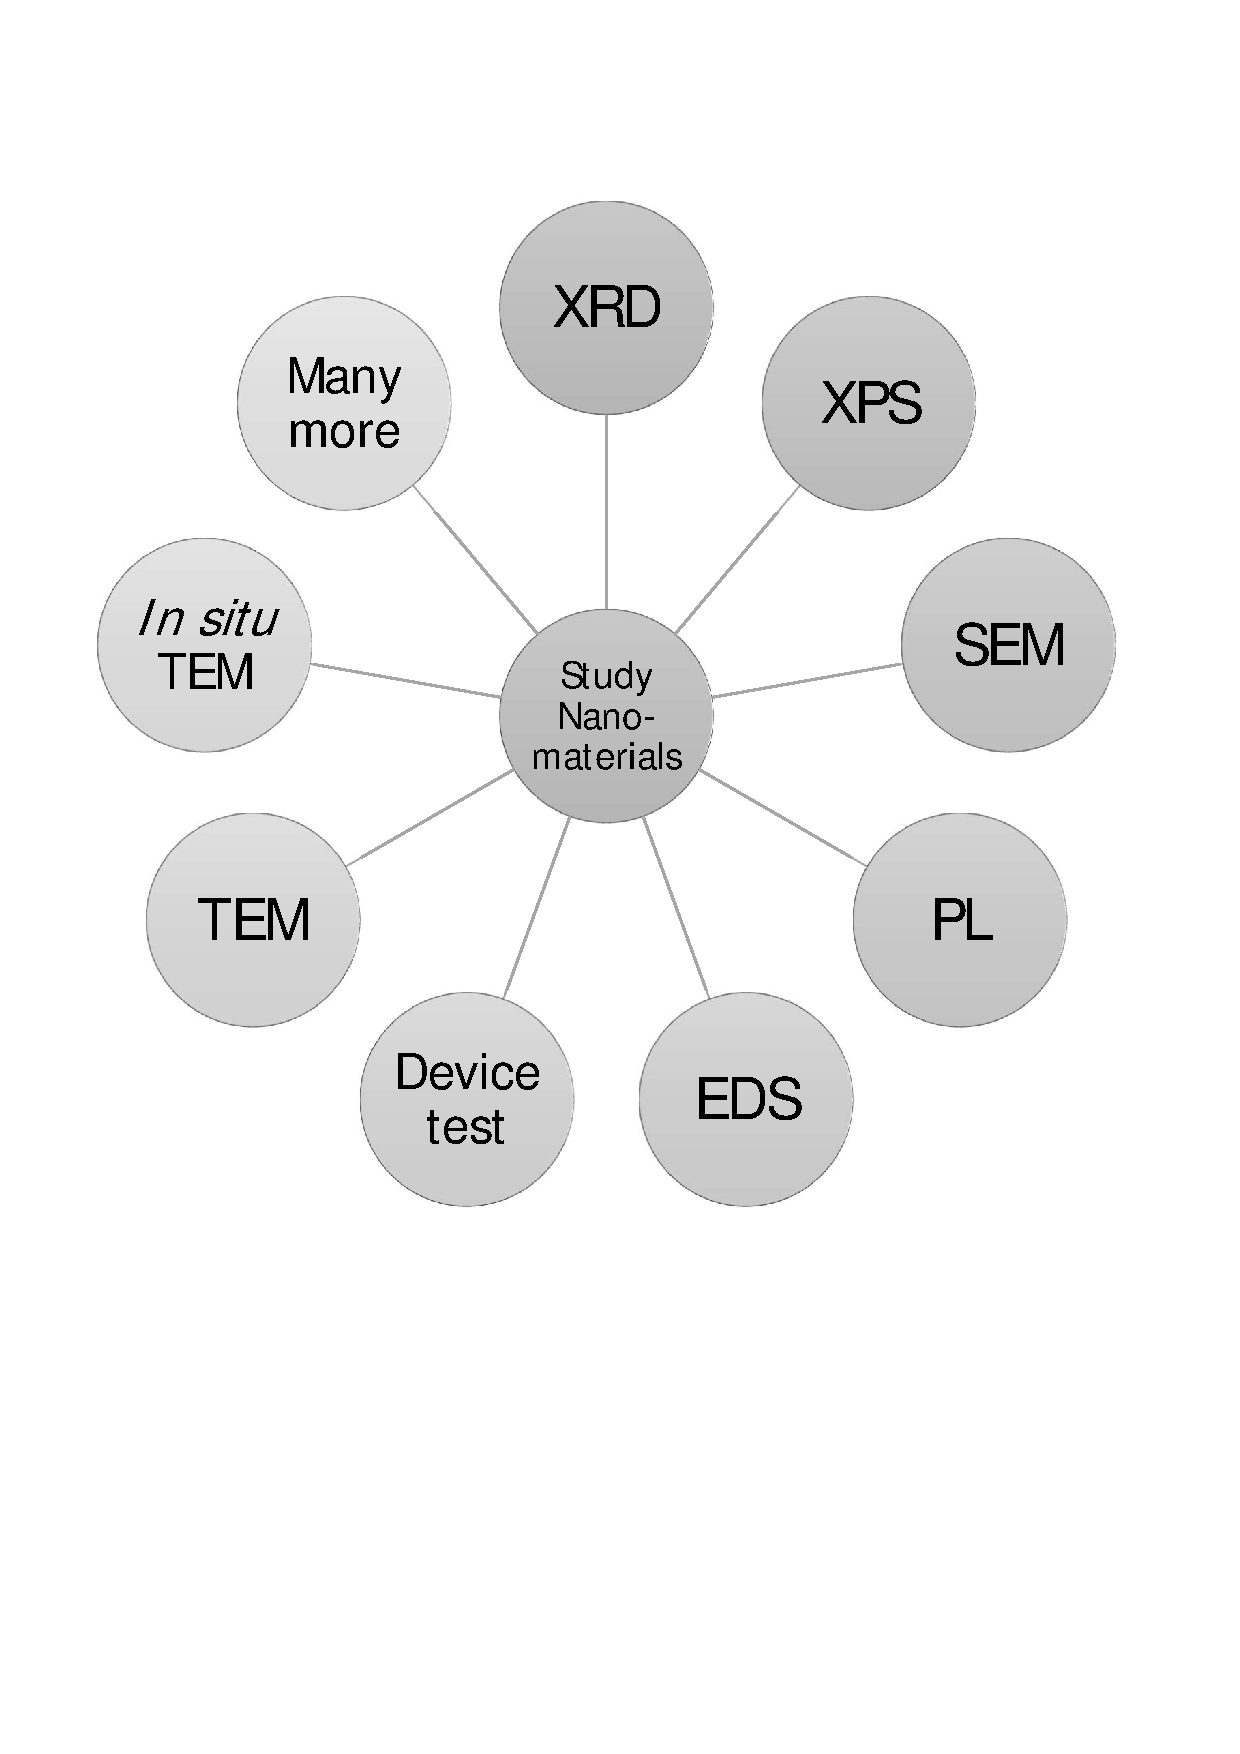
\includegraphics[width=320pt]{figures/figure1_to_study_nanomater.pdf}
\caption[Study of nanomaterials]{{\em In situ} TEM serves as a way to study nanomaterials.
\label{fig:1tsn}}
\end{figure}
%what is in situ TEM

\section{Seeing is believing: Transmission Electron Microscopy}
In the past century, development of particle physics made a way for new microscopies, such as Scanning Probe Microscopy (SPM, including Atomic Force Microscopy and Scanning Tunneling Microscopy), Scanning Electron Microscopy (SEM), and Transmission Electron Microscopy (TEM). Among all microscopies, TEM, has the best ultimate spatial resolution; this allows one to reach atomic resolution and to simultaneously get full crystallography information. TEM provides deep and direct information from a thin sample through the transmission and diffraction of electrons. 

When researchers are not satisfied with only seeing of a material in statics, dynamics may be introduced to the sample. \emph{In situ} TEM is the newest advanced technique which gives access to the sample dynamics \textit{via} observation, manipulation and various tests.\\
Particularly, by adapting the microscope or using a special specimen holder, it is possible to make deliberate attempts to modify materials during high-resolution characterizations. It allows for the observation of dynamic properties within a material under special circumstances.\cite{banhart2008situ}\\

\begin{figure}  
\centering
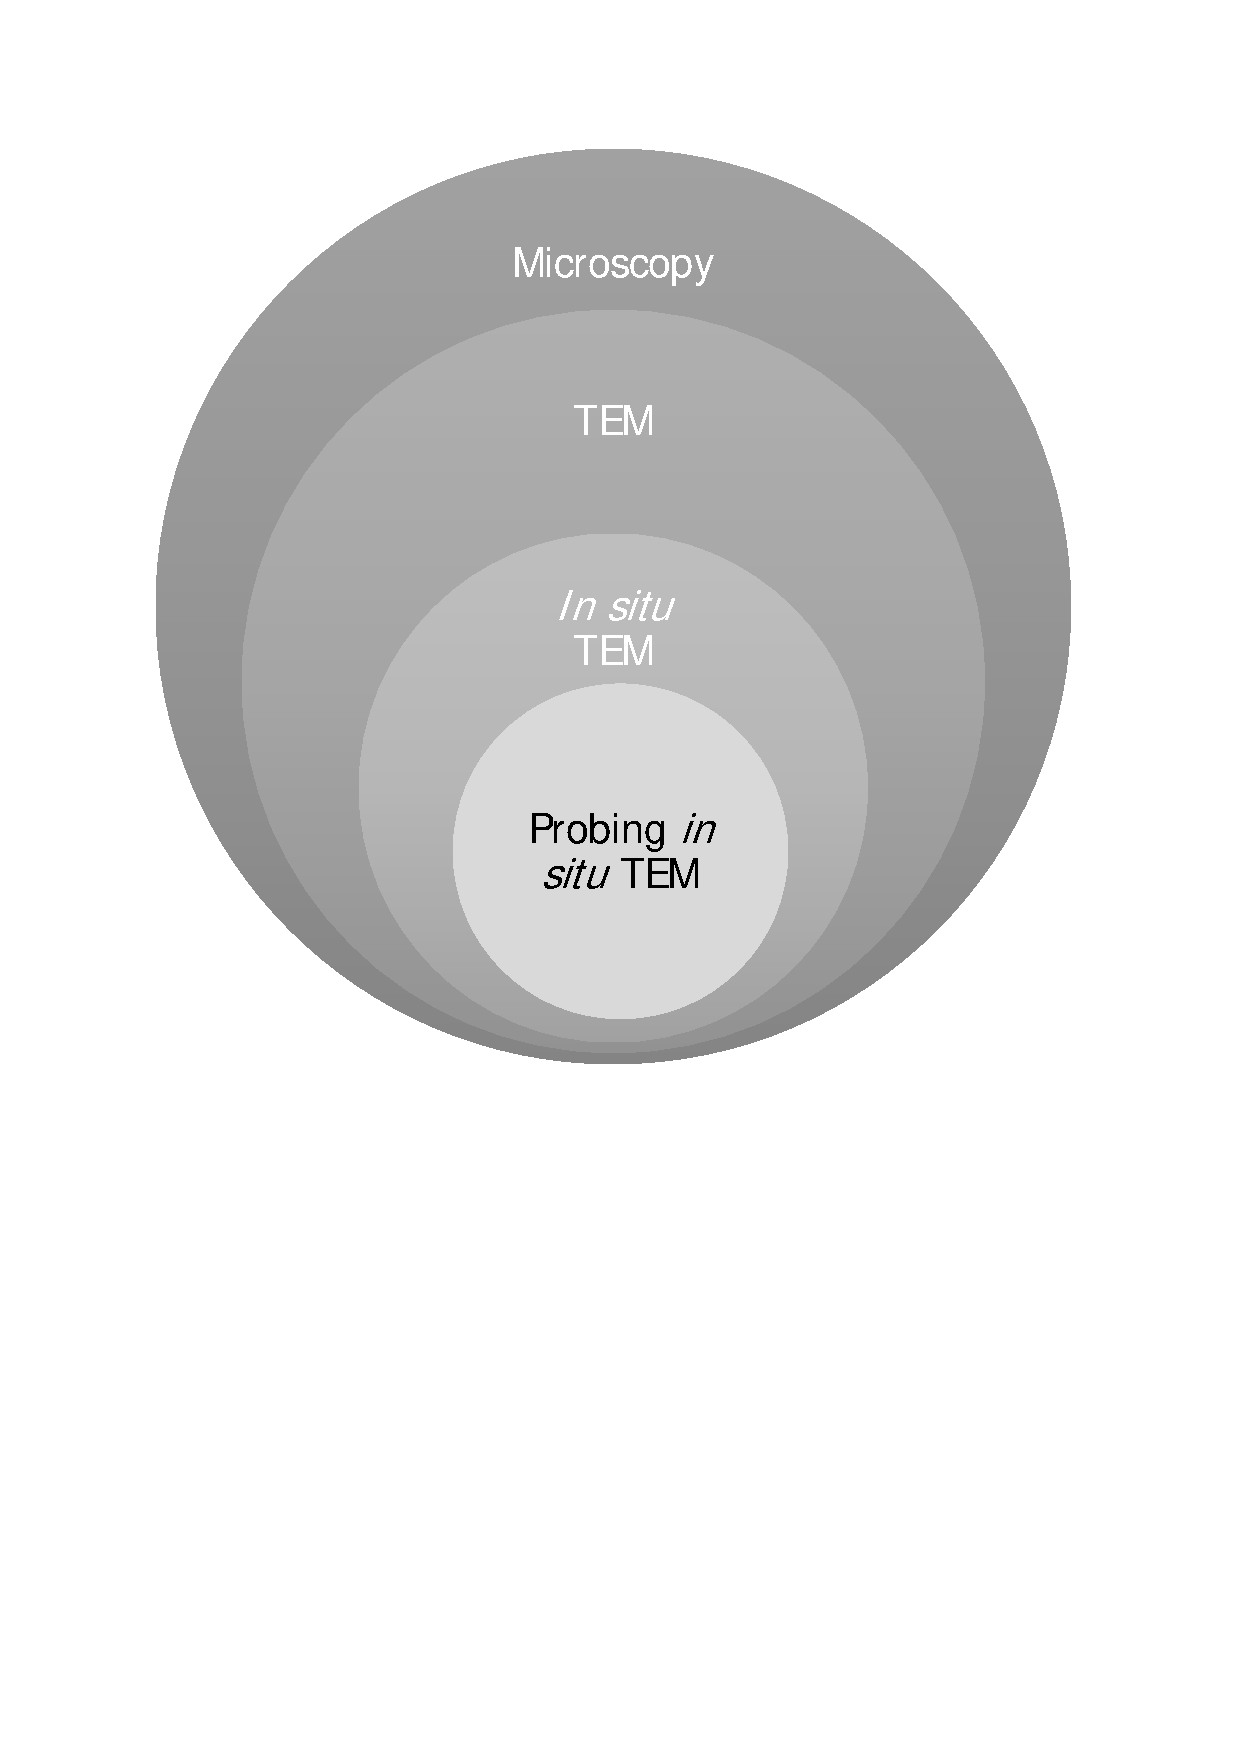
\includegraphics[width=0.6\textwidth]{figures/figure1_TEM_As_Microscopy.pdf}
\caption[\emph{In situ} TEM as a microscopy branch]{Relationships between \textit{in situ} probing TEM and other microscopies.
\label{fig:1tam}}
\end{figure}

For instance, a heating holder would provide the desired high temperature to trace (by a fast CCD video camera) and, thereby, reveal chemical transformations within a sample. By contrast, without \emph{in situ} heating, one is  only able to see the initial and final states of the reaction; in this way the regarded mechanism is usually inferred based on a few indirect clues, such as X-ray Diffraction (XRD), X-ray photoelectron spectroscopy (XPS), Energy Dispersive X-ray Spectrometry (EDS), Photoluminescence (PL) and indirect TEM characterizations before and after the dynamic tests. As illustrated in Figure \ref{fig:1tsn}, \emph{in situ} TEM is very important and irreplaceable approach to study nanomaterials. \\

Various specimen holders make it possible to introduce heating, cooling, electrical bias, mechanical force, gas, liquid, magnetic field, light etc. to the sample under various conditions. As illustrated in Figure \ref{fig:1tam}, probing \emph{in situ} TEM is one small domain of microscopy as a whole. And this dissertation is mainly focused on probing of nanomaterials \textit{via in situ} TEM. 

\section{Untouchable scale: Probing techniques for nanomaterials}

The experiments performed by \textit{in situ} probing microscopy are carried out based on piezoelectric effect and microscopy. \\

\begin{figure}  
\centering
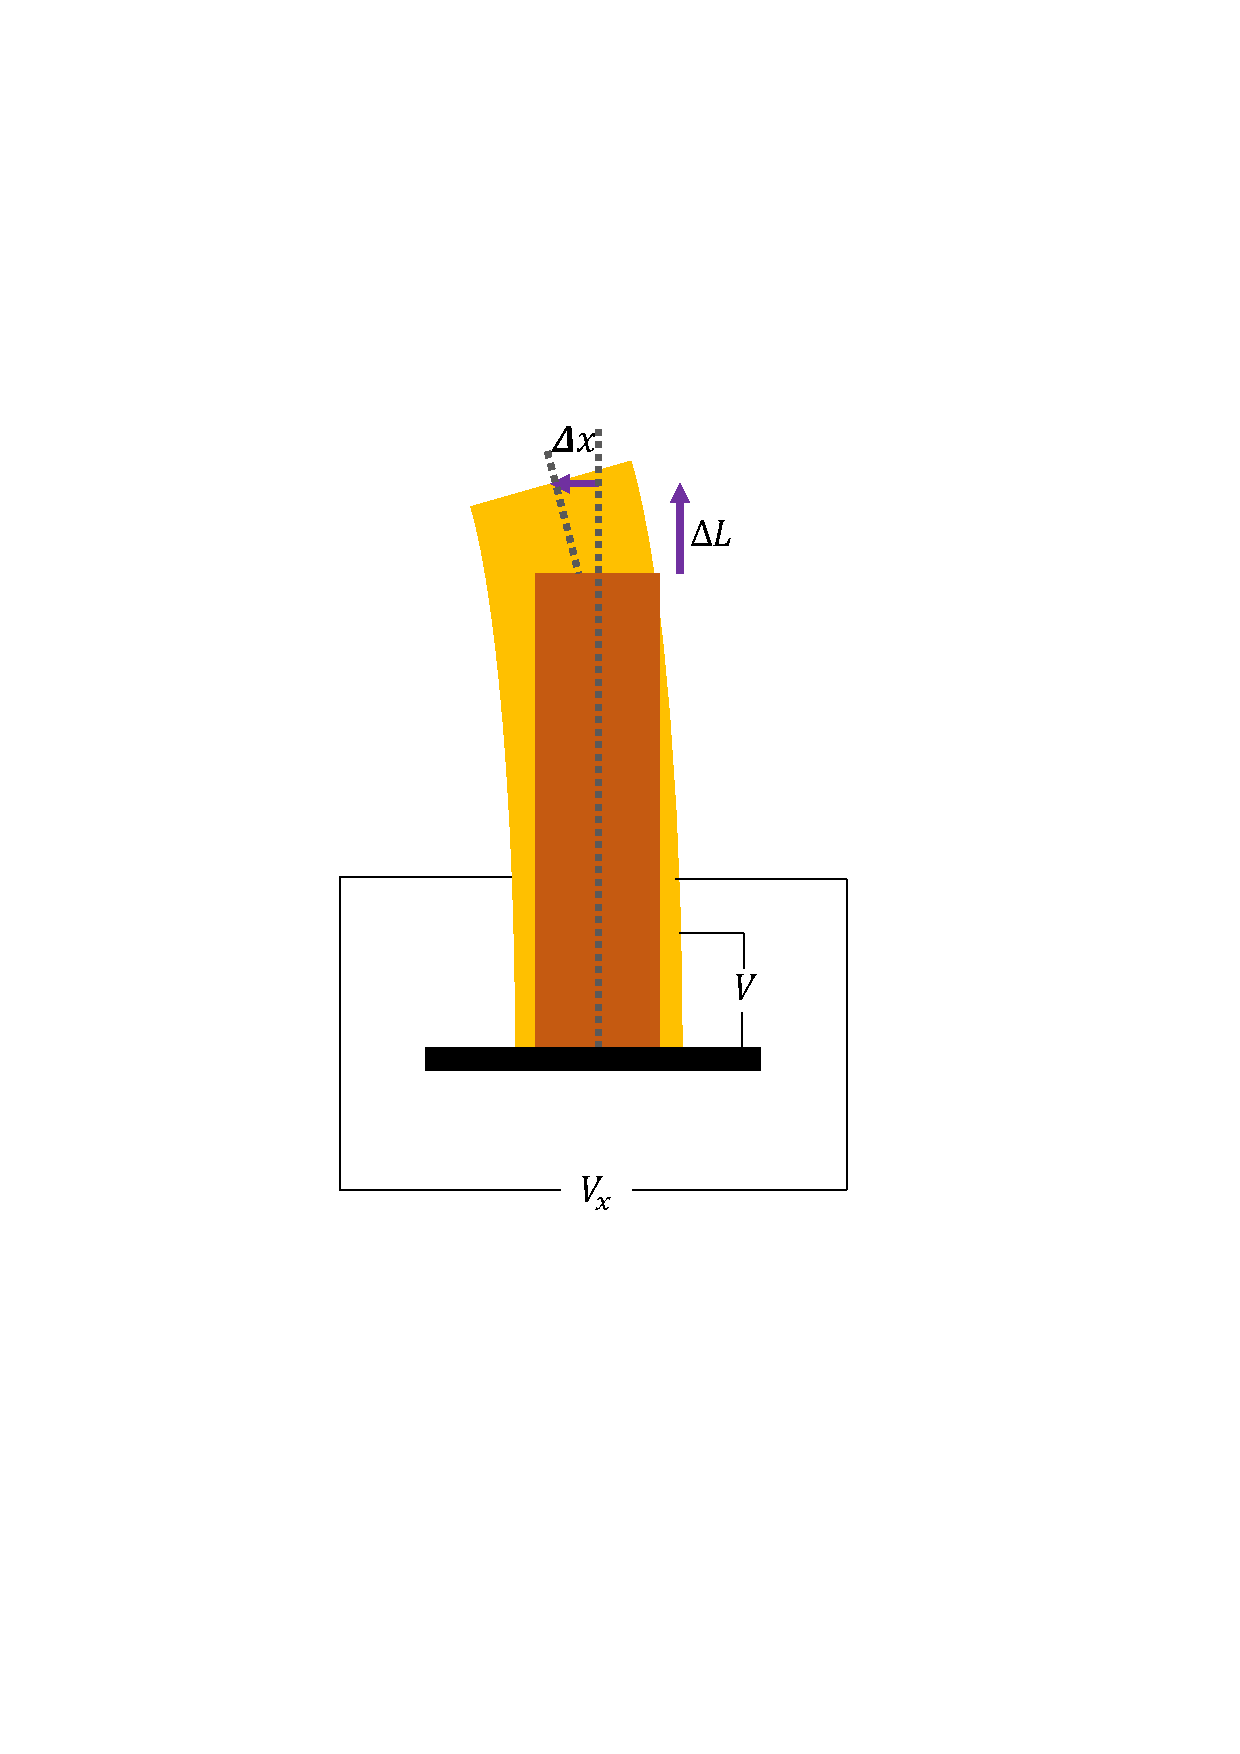
\includegraphics[width=230pt]{figures/figure1_piezo.pdf}
\caption[Probing by piezoelectronics]{Schematic illustration of how piezoelectric works for precised nanomanipulations.
\label{fig:1piezo}}
\end{figure}

Piezoelectricity is a phenomenon where electricity is directly related to the pressure applied to the material. In a piezoelectric actuator, special driving signals are applied to a piezoelectric tube in certain directions, and, thereby, the piezoelectric tube would respond while changing shape accordingly.\cite{okada2004piezoelectric,vishnevsky1977piezoelectric} As shown in Figure \ref{fig:1piezo}, when the base of the tube is fixed, transverse and axial movements of the tube tip would be expressed approximately by the following equations:
$$\begin{bmatrix}\Delta x\\ \Delta y\end{bmatrix}= \frac{2\sqrt{2}d_{31}}{\pi Dh}L^2\begin{bmatrix}U_{+x}-U_{-x}\\U_{+y}-U_{-y} \end{bmatrix},$$
$$\Delta L= \frac{d_{31}L}{h}V$$
, where $\Delta x$, $\Delta y$ and $\Delta L$ are deflections in $x$, $y$ and axial directions, $U_{+x}-U_{-x}$ , $U_{+y}-U_{-y}$ are driving voltages applied to the opposite sides of the tube (therefore in total four electrodes exist, in addition to the base ground electrode).$V$ is a voltage applied to all four quadrants. $L$, $D$ and $h$ is the length, diameter and thickness of the tube. The transverse piezoelectric coefficient $d_{31}$  is very small (about $-10^{-10} \mathrm{m/V}$), and, hence, the movement can be controlled precisely by biasing. 

With a help of a piezoelectric actuator, we can handle an ultrasharp probe to touch the nanoscale sample with the nanometer precision. 
\\
Now we have two effective ways to see and touch a nanostructure -- {\em in situ} TEM and piezo-motor-driven probing. 


\section{Optoelectronic and flexible electronic applications of nanomaterials}
%light to replace electrons
We are currently fully enjoying the benefits of well developed microelectronics and nanoelectronics. However, people are trying to improve the speed of information transmission by means of light. As compared with electrons in the metalic conductors (copper or even gold), photons in the optical system possess much higher capacity of information. The Society benefits a lot from the optical fiber information technology. For instance, it was quite difficult and expensive to perform high-definition video streaming \textit{via} Internet 20 years ago, when we were using copper wires to transmit electrical information. 
%silicon is not best for optoelectronics
The silicon-based electronics is efficient and is mainly based on the two materials: silicon and copper (or other conductors, such as gold). The manufacturing is sophisticated and requires etching silicon chips and applying a mask for electrode coating. Silicon is absolutely perfect semiconducting material. By doping techniques and smart designs, billions of transistors could work at a high speed within a nail-sized chip. The problem is (for optoelectronic applications) that the band-gap diversity is required. Therefore silicon, as a perfect semiconductor for electronics, could not realize fully functioning optoelectronics. \\ 
%silicon is not best for flexible electronics
Besides, flexible electronics attracts a great deal of attention. In the last few years, we experienced an explosion of flexible optoelectronic applications in flat-panel displays, lighting, sensing, and energy cells. For instance, organic light-emitting diodes (OLED) and flexible lithium-ion batteries are developed as the next-generation technology for wearable electronics, bendable smart-phones, foldable displays, \textit{etc.} However, to make silicon wafers flexible is never an easy task. Therefore, people believe that the bottom-up technology would be able to architect nanoscale building blocks on a flexible substrate for future flexible electronics and optoelectroncs. \\

\begin{figure}  
\centering
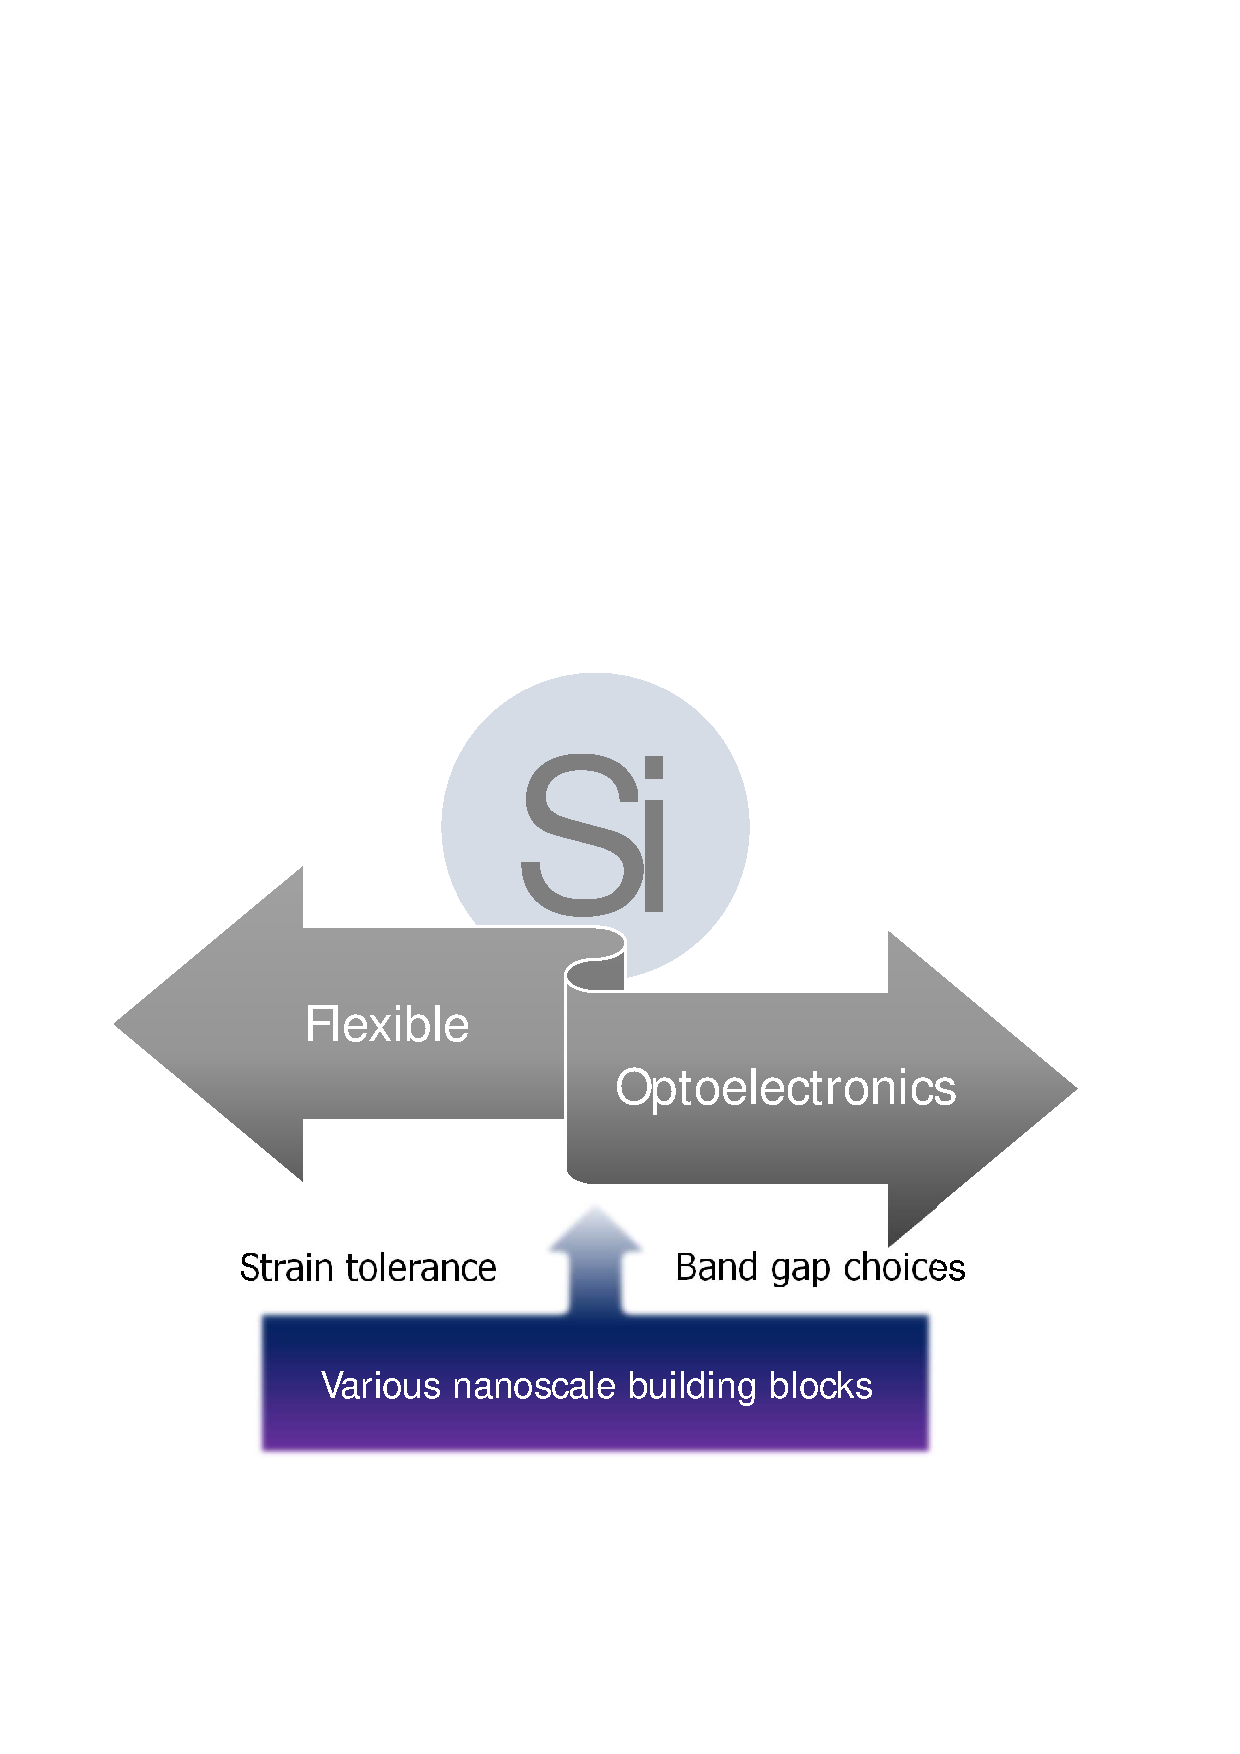
\includegraphics[width=340pt]{figures/figure1_silicon.pdf}
\caption[Future of optoelectronics and flexible electronics]{Silicon's two short-comings for flexible devices and optoelectronics could be backed-up by bottom-up approach using nanomaterials in future integrations.
\label{fig:1si}}
\end{figure}

%So nanomater is good for optoelectronics and flexible applications
Therefore, for optoelectronic and flexible electronic applications, the usage of conventional silicon industries is challenging, as shown in Figure \ref{fig:1si}. Silicon  is an ideal material to meet all requirements within a field effect transistor. The silicon based devices rely on controlling carriers realized \textit{via} structural design and doping. In recent years, silicon-based optoelectronics is growing steadily but not exponentially, as expected by Moore's Law. \cite{Waldrop2016} 
The semiconductor industries produce devices mainly by the top-down strategy. A top-down approach is a smart way to apply desired patterns to the device engineering, which came in effect since 1970s, when human beings were not so experienced to manipulate nanostructures. However, these days a bottom-up approach is emerging and shows a high promise in constructing systems by piecing building blocks together. It is true that some nanomaterials show superior properties for electronics, but it appears that during the last decade, many efforts from various research groups have been unable to establish the bottom-up technology as a real market value. \\
It is expected that in the future high quality nanomaterial building blocks could be well handled for device integrated \textit{via} the automated mass production. The integrated LDs, LEDs and photodetectors could be manufactured using nanowires, nanosheets, and even quantum dots, to realize fully functioning optoelectronic chips. The current obstacle is to get more knowledge on the building block materials. How does the electrical signal from nanowires or nanosheets behaves under strain and light illumination, what is the photocurrent spectroscopy of the material - such questions are not well studied. Consequently, it is strongly desired that we find the answers to these questions in order to provide clues for future flexible electronics and optoelectronics. 

\section{Energy storage applications of nanomaterials}
%energy is important
Electrical energy storage will be far more important nowadays than it was when we had abundant petroleum resources. From powering portable electrical devices (cell phones, tablets, laptops), implantable medical applications (pacemaker), to machines (hybrid electric vehicles), the humans' desire for clean, safe, fast and efficient energy storage is becoming more and more  significant. \\
%ion-batter is important
Among all energy storage applications, lithium ion-batteries (LIBs) are the most needed devices due to their high energy density, which is the key factor for portable electronics and automobiles. In LIBs, lithium ions move from the anode to cathode during discharge, and back during charging. The materials for the anodes and cathodes can dramatically affect the few key aspects of the battery’s performance, including its stability and capacity. High capacity materials are eagerly demanded in order to address the needs for better energy density, cycle life and charge lifespan, among other issues faced by Li-ion batteries. 
%Nanomater for ion-battery
However, conventional materials, although being  well developed,  still cannot catch up with the growing demands of battery capacity. Li-ion batteries have struggled with numerous issues, such as poor cycle life, rising internal resistance with cycling and aging, safety concerns (especially when overheated), charging speed, and limited capacity. \\
A lot of researches have confirmed that nanomaterials are particularly promising to solve these problems. The advantages are as follows\cite{Bruce2008,qifengzhang2013csr}: \\
\begin{itemize}
	\item[a] The reduced size significantly increases the rate of energy transformation between electrical and chemical energy (such as lithiation and delithiation process) due to the short diffusion lengths; 
	\item[b] Many nanomaterials enable electrode reactions to become reversible while they are not reversible for bulk materials; 
	\item[c] High surface to volume ratio provides large contact area between electrodes and electrolyte; 
	\item[d] Electron conductivity can also be improved in nanomaterials; 
	\item[e] Chemical potentials of ions and electrons can be different at the nanometer scale, and, therefore, electrode potential can be modified. 
\end{itemize}

\begin{figure}  
\centering
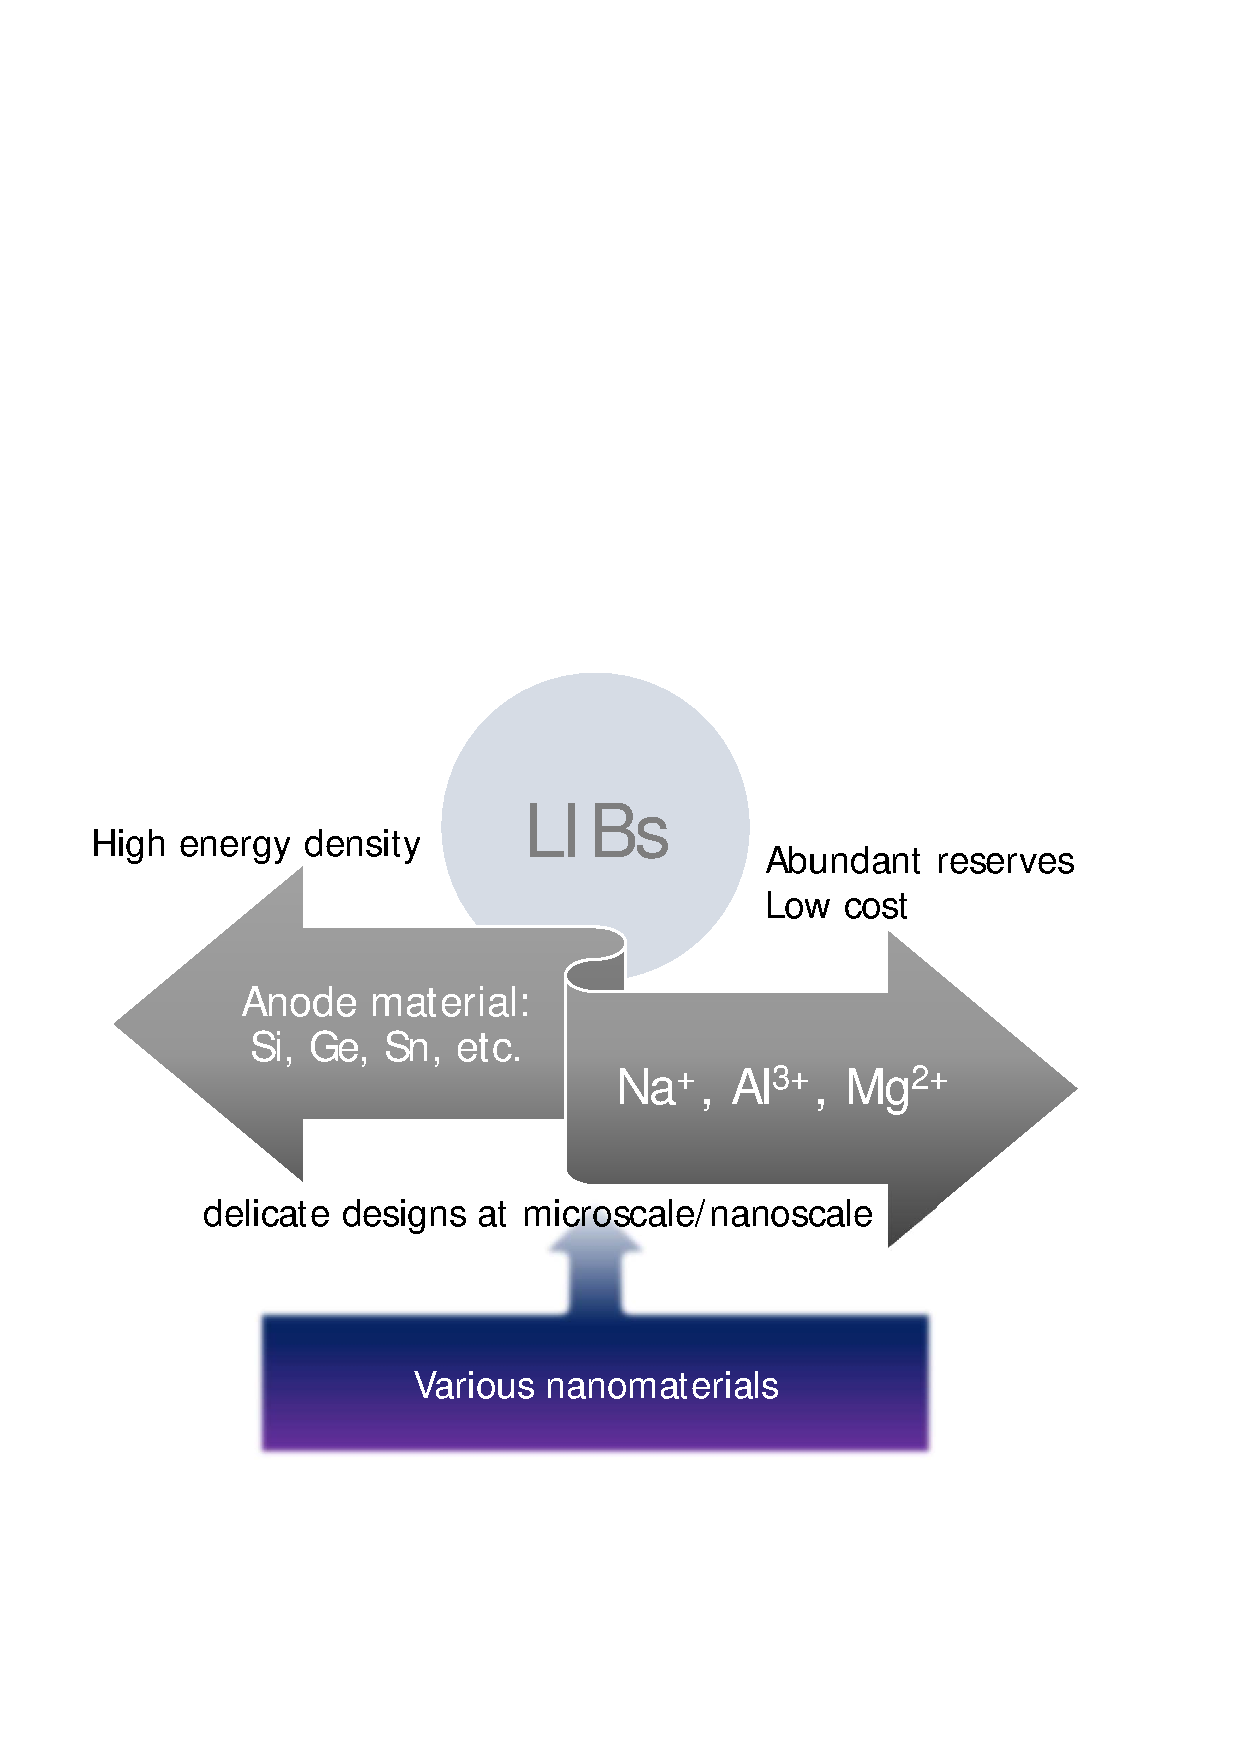
\includegraphics[width=340pt]{figures/figure1_lib.pdf}
\caption[Future of secondary ion batteries]{{A scheme showing that secondary batteries are mostly based on Lithium and graphite. However, to gain a higher energy density while using cheaper/abundant elements, nanomaterials might be the key. }
\label{fig:1lib}}
\end{figure}

%silicon for ion battery anode
 Graphite has widely been used as an anode of choice for commercial products, since the first generation of Li-ion chemistry studies appears. Due to strong needs of high capacity, in recent years, researchers have been interested in developing silicon anode materials for high capacity lithium-ion batteries. Among all investigated anode materials, silicon has one of the best  theoretical capacities of 3590 mAh/g (about 10 times higher than carbon) based on the fully alloyed form of \ce{Li15Si4} at room temperature (at high temperature \ce{Li15Si4} can be obtained, giving a capacity of 4200 mAh/g, placing it on top of all other anode materials. In addition, Si anodes show moderate working potential at $0.5$ V, which is higher than for graphite anodes at $0.05 $ V. This means that silicon is suitable to solve the safety problem of lithium deposition upon cell overcharge, as well as avert the energy penalty of battery cells assembled with the \ce{Li4Ti5O12} anodes.\\
 However, the insertion/extraction of lithium ions result in significant volume change - about 370\% - which leads to structural pulverization and electrical disconnection between anode materials and current collector, and finally the battery loses most of its functions. Some recent designs of LIBs using silicon materials as anodes allow the battery to maintain its initial anode structure and, hence, to reach high capacity and, at the same time, good stability. 

 Cui et al. a designed high performance anode structure using Si nanowires, which were able to accommodate large strains caused by lithium ion insertion and extraction.\cite{Cui2009} 
 Deng et al. reported a tubular configuration made from rolled-up C/Si/C layered nanomembranes which had performed with a highly reversible capacity at approximately 2000 mAh /g (50 mA/g), and has approximately 100\% capacity retention (500 mA/g) after 300 cycles.\cite{Deng2013}
 Cui et al. also designed core-shell structures for Si-based LIBs. They proposed a hierarchically structured Si anode which was inspired by the structure of a pomegranate. Si nanoparticles became encapsulated by conductive carbon coatings. This leaves just enough space for the expansion and contraction during lithiation and delithiation cycles. \cite{Liu2014d}
   
\begin{figure}  
\centering
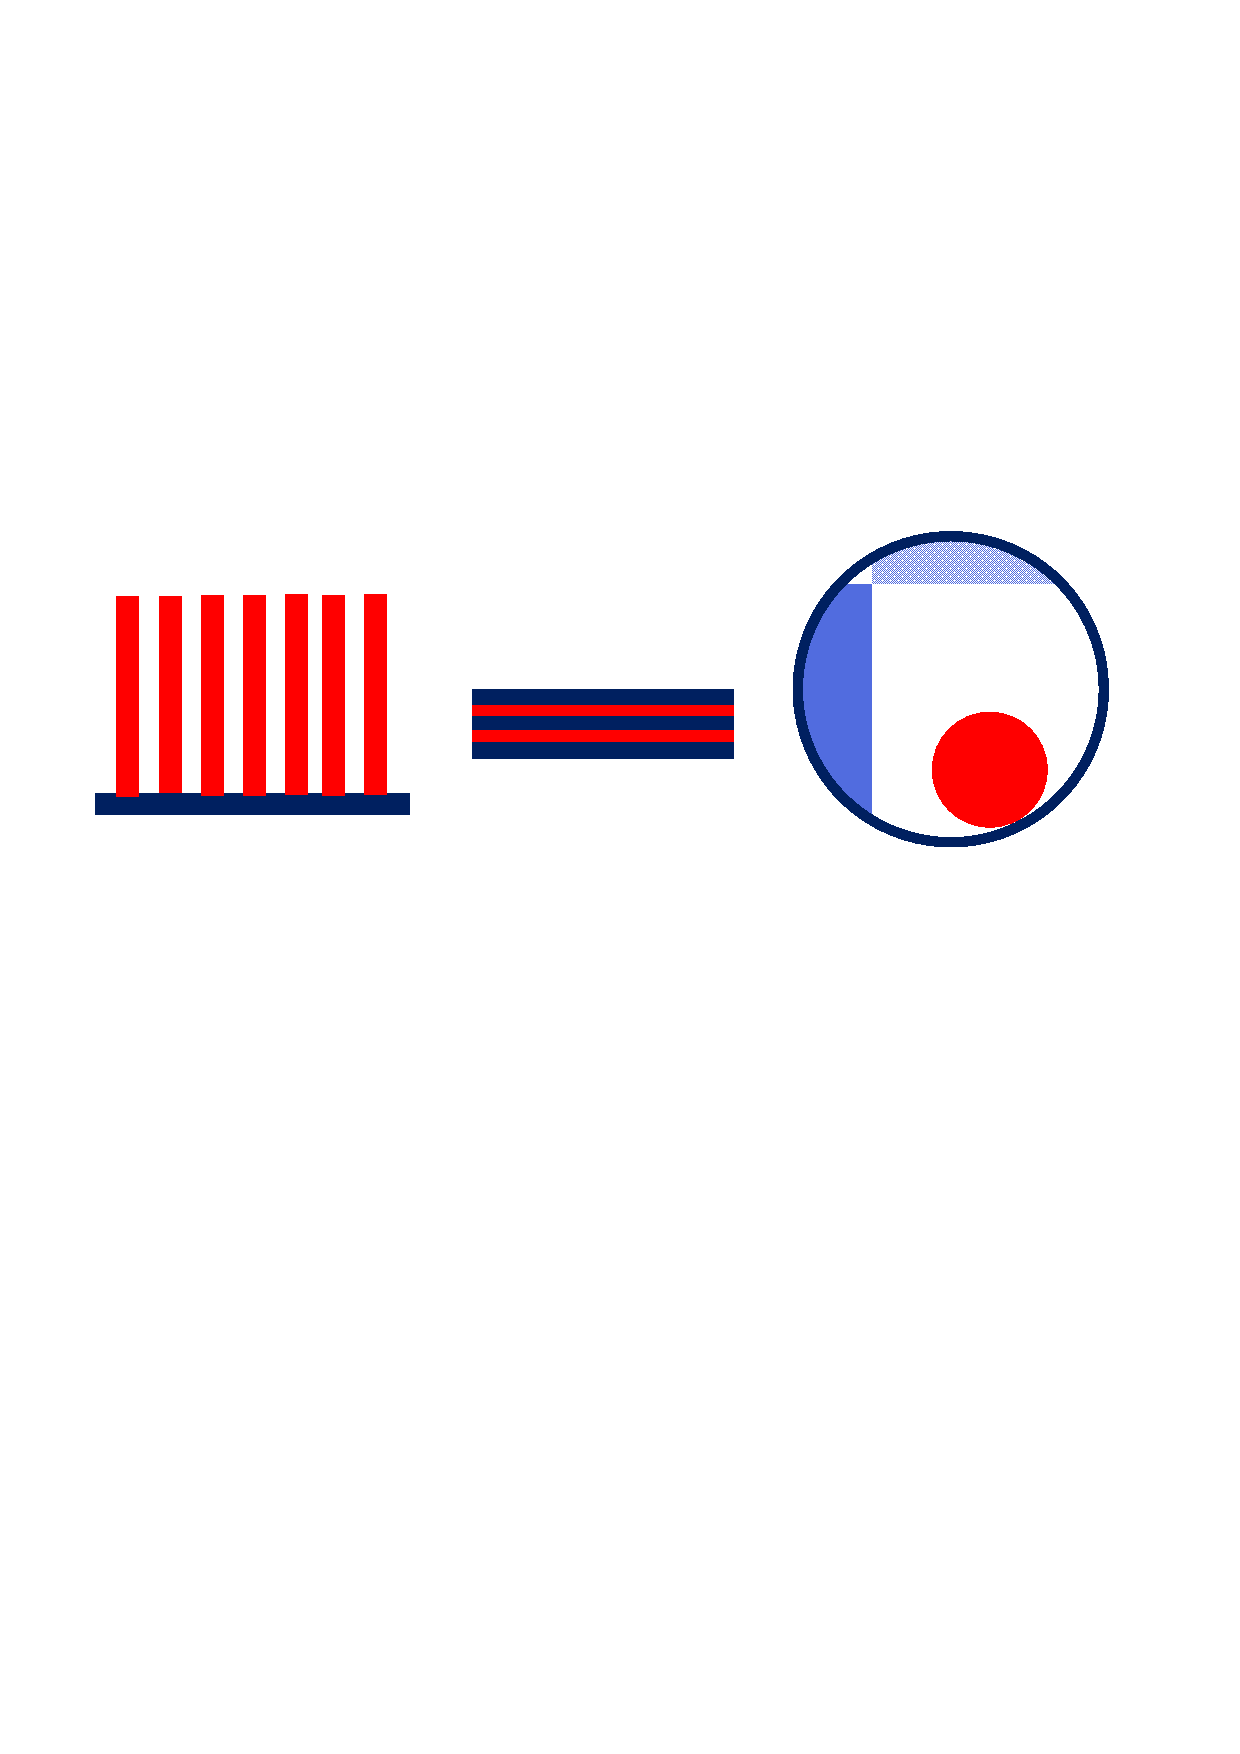
\includegraphics[width=\textwidth]{figures/figure1_silibdesign}
\caption[Designs for large volume expansion anode materials]{Designs for large volume expansion anode materials in batteries. Red correspond to material with large volume expansion/shrinking during cycling, while material in blue color is the confinement material with low volume expansion rate and good mechanical strength. 
\label{fig:1silibdesign}}
\end{figure}
 
Therefore, by designing the microscopic structures, one is able to utilize a high capacity material under structural and mechanical restrictions, as illustrated in Figure \ref{fig:1silibdesign}. Also, many other attempts of combining silicon with carbon materials,  polymers,  metals, were summarized by Liang et al.\cite{Liang2014} 
 
%Na-ion batteries
It is predicted that lithium would be the next energy resource which substitutes for petroleum, which will die out. According to the distribution of lithium on Earth\cite{Jaskula2011a}, Chile could be the next Saudi Arabia it terms of richness of resources. This problem is more severe for many countries with very limited lithium reserves, such as Japan. \\
In order to explore the next generation of secondary batteries, which are called post-lithium ion secondary batteries, many investigations
show that the most promising candidate is the sodium-ion battery (SIB). SIBs use sodium instead of lithium as the charge carrier, and use iron, manganese and other transition metals to replace cobalt for redox reactions. SIBs are expected to be mass produced in the nearest future due to their minor environmental impacts and a relatively low cost.

\begin{table}[ht]
\centering % used for centering table
\begin{tabular}{|l|c|c|} % left, centered columns (3 columns)
\hline %inserts double horizontal lines
 & LIB & SIB\\ [0.5ex] % inserts table heading
\hline % inserts single horizontal line
Theoretical capacity & 3,829 mAh/g & 1,165 mAh/g \\[1.5ex] % inserting body of the table
Cost (carbonate) & 5,000 USD/t & 150 USD/t \\[1.5ex]% [1.5ex] adds vertical space
Reserves & 23,000 ppm & 20 ppm \\[1.5ex]
Potential & –3.045 V & –2.714 V \\[1.5ex]
Ionic radii & 79.3 pm & 100.9 pm \\[1.5ex]
\hline %inserts single line
\end{tabular}
\caption{Comparison of LIB with SIB.} % title of Table
\label{table1.1} % is used to refer this table in the text
\end{table}

As shown in Table \ref{table1.1}, although sodium possesses a higher normal electrode potential of ~0.3 V, larger effective radius than lithium (in volume ratio 2.05), and smaller theoretical capacity, its cost and environmental benefits are still very attractive for applications which do not require very high capacity. Actually, it is hard for graphite, which is commercially used as an anode material for LIBs, to store and release sodium ions both theoretically and in practice because the sodium ion size is large. \\
However, it was discovered in 2000 that hard carbon having disordered structures could electrochemically store and release sodium ions.\cite{Stevens2000} Several years ago, a work was done on developing and making practical sodium ion batteries, and since recently researchers have been investigating on many anode active materials for sodium ions. It is worth noting that well-established guidelines and experiences acquired for LIBs electrode active materials are not applicable for SIBs.\cite{Lang2010,Armand2008,KUZE2013}

Consequently, the two currently important research areas for secondary batteries are: finding better anode active materials with higher capacities, and looking for other elements for ion batteries, as illustrated in Figure \ref{fig:1lib}. To apply these elements in secondary batteries, nanomaterials, or nanoscaled designs play very important roles. They enable reactions which may overcome huge volume expansion and decrease diffusion lengths; while bulk materials are not capable to reach the highest capacity either for LIBs or for other special ion-batteries at the moment. 

\section{Motivation of my PhD research}
As stated above, {\em in situ} studies on nanomaterials toward optoelectronics, electronics and ion batteries are required by the Society. My motivation is to take the challenge and to analyze the dynamics of the building blocks, as well as heterostructures, and to provide decent knowledge for advanced applications. 
Therefore, I explored some experimental methods and engineering details, including {\em in situ} TEM setups and the working mechanisms. \\
Then, I present manipulation possibilities in the frame of the general \textit{nanoarchitectonics} concept and its applications for nanoengineering. The experiments have been performed on the {\em in situ} TEM-constructed axial nanowire junctions of CdS and p-Si. In addition, detailed electrical probing for energy storage research is discussed. I fabricated an ultra-stable sodium ion battery and analyzed the mechanism of its cycling performance under {\em in situ} TEM probing. Through coupling with {\em in situ} TEM applied mechanical forces, two examples of force-driven optoelectronic phenomena are detailed taking the examples of ZnO and CdS. 